% Options for packages loaded elsewhere
\PassOptionsToPackage{unicode}{hyperref}
\PassOptionsToPackage{hyphens}{url}
%
\documentclass[
]{article}
\usepackage{amsmath,amssymb}
\usepackage{iftex}
\ifPDFTeX
  \usepackage[T1]{fontenc}
  \usepackage[utf8]{inputenc}
  \usepackage{textcomp} % provide euro and other symbols
\else % if luatex or xetex
  \usepackage{unicode-math} % this also loads fontspec
  \defaultfontfeatures{Scale=MatchLowercase}
  \defaultfontfeatures[\rmfamily]{Ligatures=TeX,Scale=1}
\fi
\usepackage{lmodern}
\ifPDFTeX\else
  % xetex/luatex font selection
\fi
% Use upquote if available, for straight quotes in verbatim environments
\IfFileExists{upquote.sty}{\usepackage{upquote}}{}
\IfFileExists{microtype.sty}{% use microtype if available
  \usepackage[]{microtype}
  \UseMicrotypeSet[protrusion]{basicmath} % disable protrusion for tt fonts
}{}
\makeatletter
\@ifundefined{KOMAClassName}{% if non-KOMA class
  \IfFileExists{parskip.sty}{%
    \usepackage{parskip}
  }{% else
    \setlength{\parindent}{0pt}
    \setlength{\parskip}{6pt plus 2pt minus 1pt}}
}{% if KOMA class
  \KOMAoptions{parskip=half}}
\makeatother
\usepackage{xcolor}
\usepackage[margin=1in]{geometry}
\usepackage{color}
\usepackage{fancyvrb}
\newcommand{\VerbBar}{|}
\newcommand{\VERB}{\Verb[commandchars=\\\{\}]}
\DefineVerbatimEnvironment{Highlighting}{Verbatim}{commandchars=\\\{\}}
% Add ',fontsize=\small' for more characters per line
\usepackage{framed}
\definecolor{shadecolor}{RGB}{248,248,248}
\newenvironment{Shaded}{\begin{snugshade}}{\end{snugshade}}
\newcommand{\AlertTok}[1]{\textcolor[rgb]{0.94,0.16,0.16}{#1}}
\newcommand{\AnnotationTok}[1]{\textcolor[rgb]{0.56,0.35,0.01}{\textbf{\textit{#1}}}}
\newcommand{\AttributeTok}[1]{\textcolor[rgb]{0.13,0.29,0.53}{#1}}
\newcommand{\BaseNTok}[1]{\textcolor[rgb]{0.00,0.00,0.81}{#1}}
\newcommand{\BuiltInTok}[1]{#1}
\newcommand{\CharTok}[1]{\textcolor[rgb]{0.31,0.60,0.02}{#1}}
\newcommand{\CommentTok}[1]{\textcolor[rgb]{0.56,0.35,0.01}{\textit{#1}}}
\newcommand{\CommentVarTok}[1]{\textcolor[rgb]{0.56,0.35,0.01}{\textbf{\textit{#1}}}}
\newcommand{\ConstantTok}[1]{\textcolor[rgb]{0.56,0.35,0.01}{#1}}
\newcommand{\ControlFlowTok}[1]{\textcolor[rgb]{0.13,0.29,0.53}{\textbf{#1}}}
\newcommand{\DataTypeTok}[1]{\textcolor[rgb]{0.13,0.29,0.53}{#1}}
\newcommand{\DecValTok}[1]{\textcolor[rgb]{0.00,0.00,0.81}{#1}}
\newcommand{\DocumentationTok}[1]{\textcolor[rgb]{0.56,0.35,0.01}{\textbf{\textit{#1}}}}
\newcommand{\ErrorTok}[1]{\textcolor[rgb]{0.64,0.00,0.00}{\textbf{#1}}}
\newcommand{\ExtensionTok}[1]{#1}
\newcommand{\FloatTok}[1]{\textcolor[rgb]{0.00,0.00,0.81}{#1}}
\newcommand{\FunctionTok}[1]{\textcolor[rgb]{0.13,0.29,0.53}{\textbf{#1}}}
\newcommand{\ImportTok}[1]{#1}
\newcommand{\InformationTok}[1]{\textcolor[rgb]{0.56,0.35,0.01}{\textbf{\textit{#1}}}}
\newcommand{\KeywordTok}[1]{\textcolor[rgb]{0.13,0.29,0.53}{\textbf{#1}}}
\newcommand{\NormalTok}[1]{#1}
\newcommand{\OperatorTok}[1]{\textcolor[rgb]{0.81,0.36,0.00}{\textbf{#1}}}
\newcommand{\OtherTok}[1]{\textcolor[rgb]{0.56,0.35,0.01}{#1}}
\newcommand{\PreprocessorTok}[1]{\textcolor[rgb]{0.56,0.35,0.01}{\textit{#1}}}
\newcommand{\RegionMarkerTok}[1]{#1}
\newcommand{\SpecialCharTok}[1]{\textcolor[rgb]{0.81,0.36,0.00}{\textbf{#1}}}
\newcommand{\SpecialStringTok}[1]{\textcolor[rgb]{0.31,0.60,0.02}{#1}}
\newcommand{\StringTok}[1]{\textcolor[rgb]{0.31,0.60,0.02}{#1}}
\newcommand{\VariableTok}[1]{\textcolor[rgb]{0.00,0.00,0.00}{#1}}
\newcommand{\VerbatimStringTok}[1]{\textcolor[rgb]{0.31,0.60,0.02}{#1}}
\newcommand{\WarningTok}[1]{\textcolor[rgb]{0.56,0.35,0.01}{\textbf{\textit{#1}}}}
\usepackage{graphicx}
\makeatletter
\def\maxwidth{\ifdim\Gin@nat@width>\linewidth\linewidth\else\Gin@nat@width\fi}
\def\maxheight{\ifdim\Gin@nat@height>\textheight\textheight\else\Gin@nat@height\fi}
\makeatother
% Scale images if necessary, so that they will not overflow the page
% margins by default, and it is still possible to overwrite the defaults
% using explicit options in \includegraphics[width, height, ...]{}
\setkeys{Gin}{width=\maxwidth,height=\maxheight,keepaspectratio}
% Set default figure placement to htbp
\makeatletter
\def\fps@figure{htbp}
\makeatother
\setlength{\emergencystretch}{3em} % prevent overfull lines
\providecommand{\tightlist}{%
  \setlength{\itemsep}{0pt}\setlength{\parskip}{0pt}}
\setcounter{secnumdepth}{5}
\usepackage{float} \floatplacement{figure}{H} \usepackage{caption} \captionsetup[figure]{font=scriptsize}
\usepackage{booktabs}
\usepackage{longtable}
\usepackage{array}
\usepackage{multirow}
\usepackage{wrapfig}
\usepackage{float}
\usepackage{colortbl}
\usepackage{pdflscape}
\usepackage{tabu}
\usepackage{threeparttable}
\usepackage{threeparttablex}
\usepackage[normalem]{ulem}
\usepackage{makecell}
\usepackage{xcolor}
\ifLuaTeX
  \usepackage{selnolig}  % disable illegal ligatures
\fi
\IfFileExists{bookmark.sty}{\usepackage{bookmark}}{\usepackage{hyperref}}
\IfFileExists{xurl.sty}{\usepackage{xurl}}{} % add URL line breaks if available
\urlstyle{same}
\hypersetup{
  pdftitle={STA2005S - Regression Assignment},
  pdfkeywords={Programming Languages, Efficieny, Large-Scaled Iterative
Compuations},
  hidelinks,
  pdfcreator={LaTeX via pandoc}}

\title{STA2005S - Regression Assignment}
\author{true \and true}
\date{2024-10-18}

\begin{document}
\maketitle
\begin{abstract}
In this report, we explored the efficiency of 6 programming languages
through the approximation of \(\pi\). We found that efficiency of
various programming languages can vary widely, with C and C++ being the
most efficient programming languages. We also presented evidence for
compiled languages having better performance than interpreted languages.
Our results suggest that programmers can benefit from taking the
efficiency of various programming languages into account, rather than
simply opting for simplicity in the syntax of these languages .
\end{abstract}

\newpage

\hypertarget{part-one-analysis}{%
\section{Part One : Analysis}\label{part-one-analysis}}

\hypertarget{section-1-introduction}{%
\subsection{Section 1: Introduction}\label{section-1-introduction}}

Air pollution, particularly high levels of particulate matter (PM), is a
major environmental and public health issue in South Africa's urban
centers. Exposure to elevated PM levels is linked to respiratory
diseases and other serious health conditions. Understanding the factors
influencing PM concentrations is crucial for developing policies that
improve air quality and protect public health. This analysis seeks to
identify the key drivers of air pollution in South Africa's cities,
focusing on how various urban, environmental, and socioeconomic factors
affect particulate matter levels.

Unknown Factors to Investigate:

Traffic Density: How do varying levels of vehicle traffic contribute to
PM levels in different areas?

Industrial Activity: What is the impact of industrial activity near
monitoring stations on air quality?

Temperature \& Humidity: How do changes in weather conditions, like
temperature and humidity, influence PM concentrations?

Wind Speed: How does wind speed affect the dispersion or accumulation of
particulate matter in urban areas?

Day of the Week \& Public Holidays: Do patterns of human activity on
weekdays, weekends, and holidays significantly influence pollution
levels?

Urban Greenery: How effective are green spaces in reducing air pollution
in densely populated areas?

\hypertarget{objective}{%
\section{Objective}\label{objective}}

The goal of this analysis is to explore the relationships between PM
levels and these explanatory variables. By identifying the most
influential factors, we aim to inform urban planning and public health
strategies that address air pollution and improve the quality of life in
South African cities.

\hypertarget{section-2-data-exploration}{%
\subsection{Section 2 : Data
Exploration}\label{section-2-data-exploration}}

\hypertarget{density-plot}{%
\subsubsection{Density plot}\label{density-plot}}

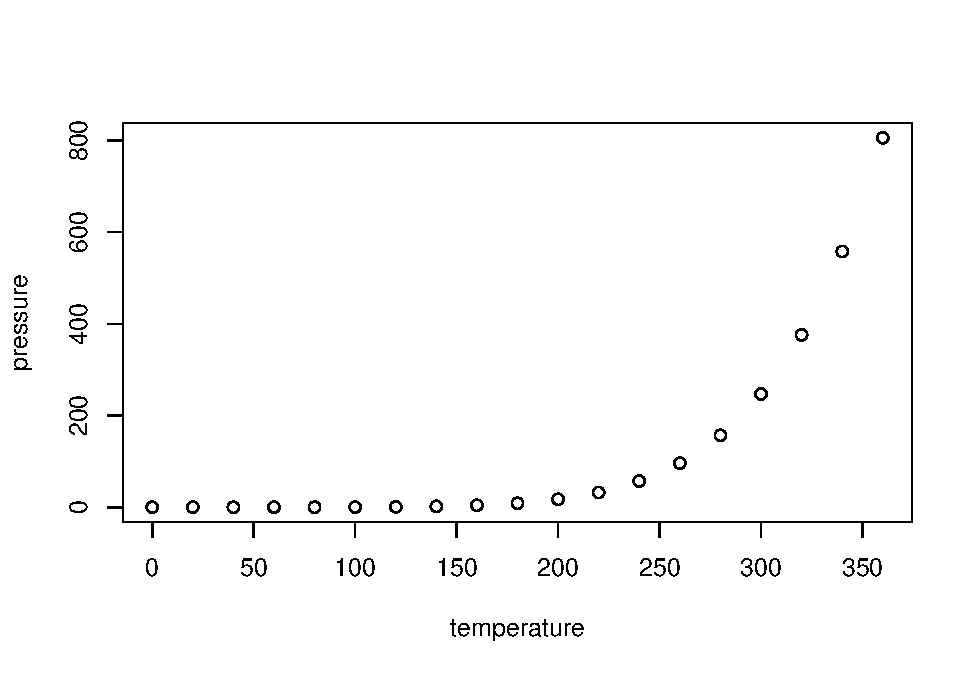
\includegraphics{Report_files/figure-latex/pressure-1.pdf}

\hypertarget{pairwsie-plots}{%
\subsubsection{Pairwsie Plots}\label{pairwsie-plots}}

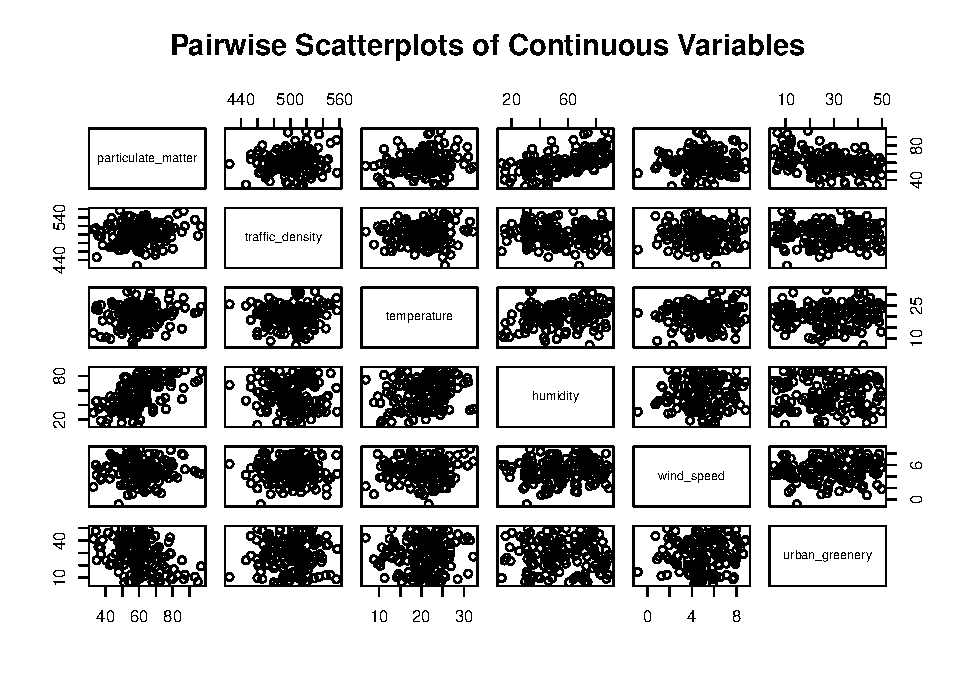
\includegraphics{Report_files/figure-latex/unnamed-chunk-1-1.pdf}

\hypertarget{categorial-variable-plots}{%
\subsubsection{Categorial Variable
Plots}\label{categorial-variable-plots}}

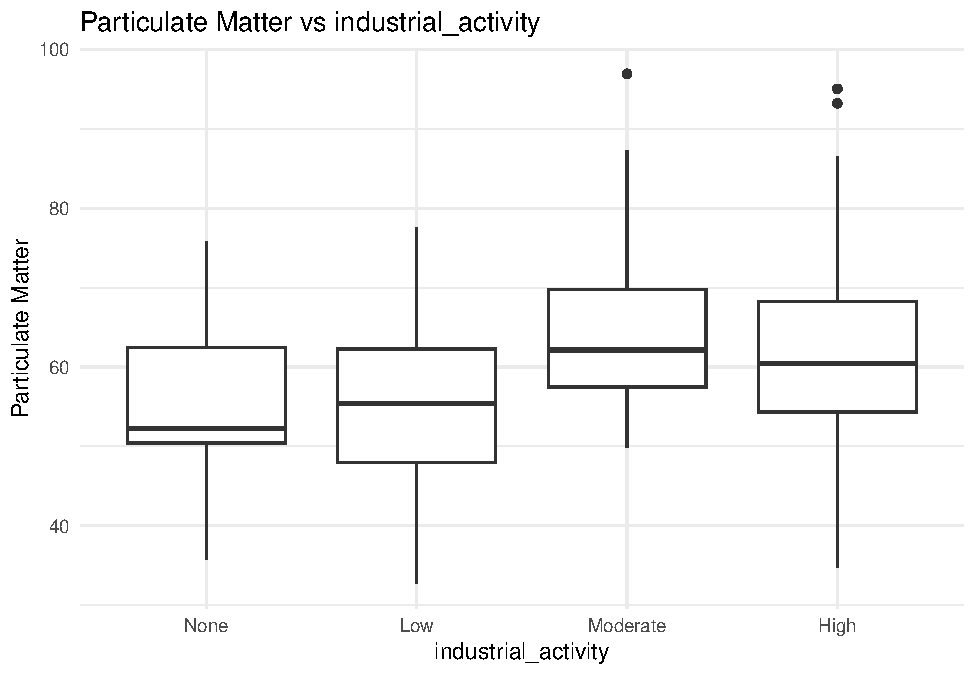
\includegraphics{Report_files/figure-latex/unnamed-chunk-2-1.pdf}
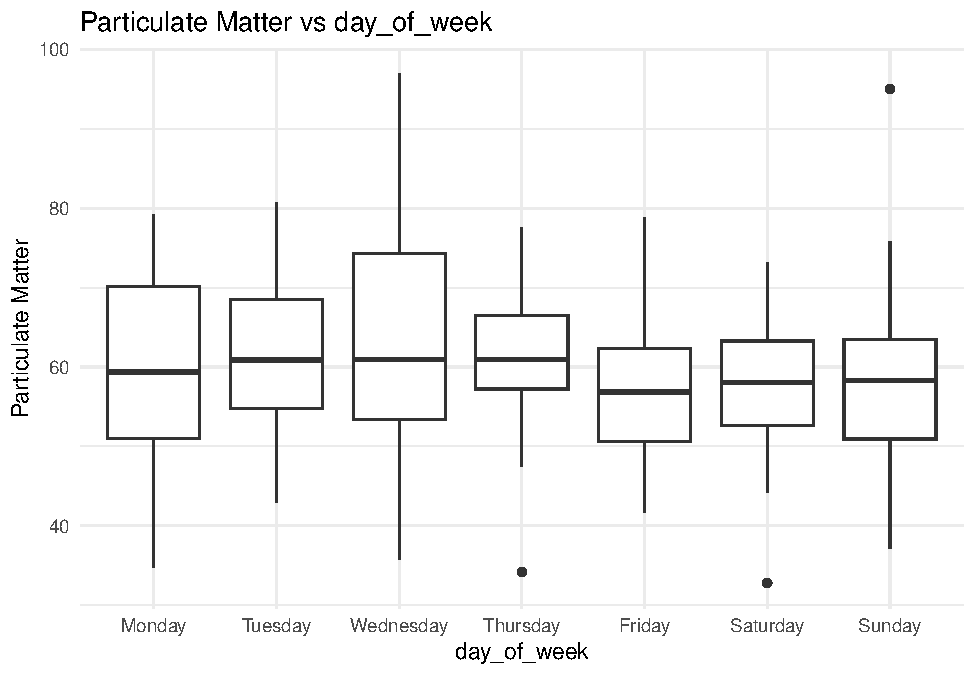
\includegraphics{Report_files/figure-latex/unnamed-chunk-2-2.pdf}
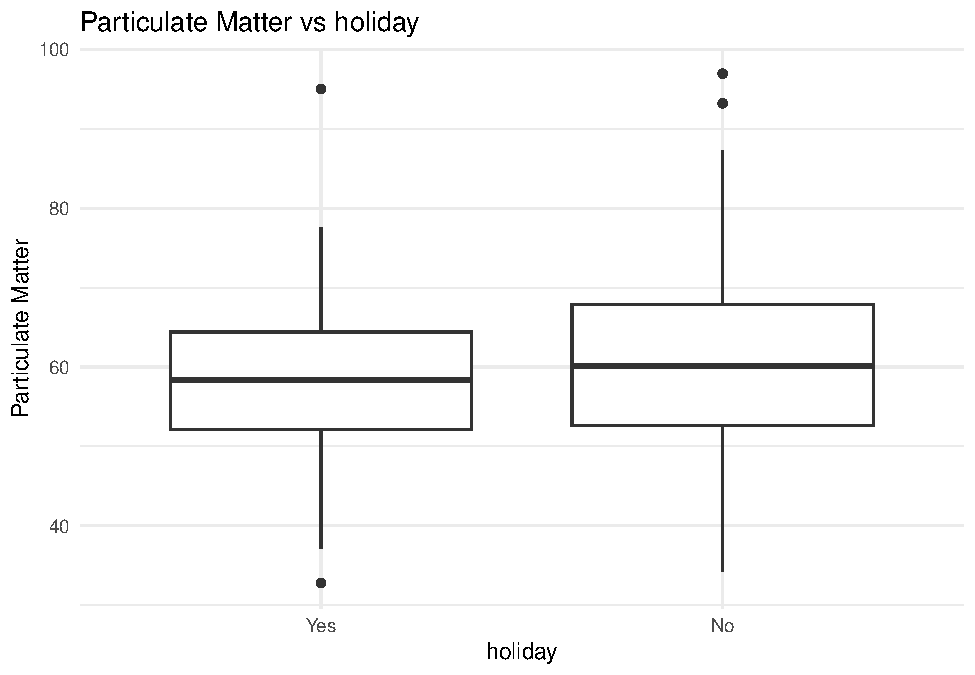
\includegraphics{Report_files/figure-latex/unnamed-chunk-2-3.pdf}

\hypertarget{visual-representation-of-relationship-between-categorial-variables}{%
\subsubsection{Visual Representation of Relationship between Categorial
Variables}\label{visual-representation-of-relationship-between-categorial-variables}}

\includegraphics{Report_files/figure-latex/unnamed-chunk-3-1.pdf}
\includegraphics{Report_files/figure-latex/unnamed-chunk-3-2.pdf}
\includegraphics{Report_files/figure-latex/unnamed-chunk-3-3.pdf}

\hypertarget{comments}{%
\subsubsection{Comments}\label{comments}}

Distribution characterisitcs:

The distribution of particulate matter levels is generally right-skewed,
indicating that a small number of observations have significantly high
levels of particulate matter while most observations are clustered at
lower levels. The presence of outliers suggests variations in local
conditions affecting air quality.

Observed Relationships

\begin{enumerate}
\def\labelenumi{\arabic{enumi}.}
\item
  Traffic Density: A positive correlation exists between particulate
  matter levels and traffic density, suggesting that areas with higher
  vehicle traffic tend to experience elevated levels of particulate
  matter.
\item
  Urban Greenery: A negative trend is observed, where higher urban
  greenery correlates with lower particulate matter, indicating that
  vegetation may help mitigate air pollution.
\item
  Temperature and Wind Speed: No strong relationship was identified
  between particulate matter and temperature. However, there is a slight
  negative correlation with wind speed, indicating that higher wind
  speeds may help disperse particulate matter.
\end{enumerate}

Potential Collinearity

Some potential collinearity is observed among the explanatory variables,
particularly between traffic density and urban greenery. High traffic
areas often have less vegetation, leading to a relationship that may
confound the analysis. Additionally, temperature and wind speed may also
exhibit collinearity, as changes in one could affect the other.

\hypertarget{section-3}{%
\section{Section 3}\label{section-3}}

\hypertarget{simple-linear-regression}{%
\subsection{Simple linear regression}\label{simple-linear-regression}}

\begin{verbatim}
## Coefficients:
\end{verbatim}

\begin{verbatim}
##                    Estimate  Std..Error   t.value Pr...t..
## (Intercept)     18.11537490 20.09831036 0.9013382 0.368873
## traffic_density  0.08399671  0.04009467 2.0949596 0.368873
\end{verbatim}

\begin{verbatim}
## 
## Residual standard error: 11.81779 on 1 and 148 DF
\end{verbatim}

\begin{verbatim}
## 
## Multiple R-squared: 0.02803719 Adjusted R-Squared:  0.02146987
\end{verbatim}

\begin{verbatim}
## 
## F-statistic: 4.269201 on 1 and 148 DF
\end{verbatim}

\hypertarget{hpothesis-test}{%
\subsection{Hpothesis Test}\label{hpothesis-test}}

\begin{Shaded}
\begin{Highlighting}[]
\CommentTok{\# Calculate F{-}statistic and p{-}value manually}
\NormalTok{group\_means }\OtherTok{\textless{}{-}} \FunctionTok{tapply}\NormalTok{(data\_tidy\_air\_quality}\SpecialCharTok{$}\NormalTok{particulate\_matter,}
\NormalTok{                      data\_tidy\_air\_quality}\SpecialCharTok{$}\NormalTok{industrial\_activity, mean)}
\NormalTok{overall\_mean }\OtherTok{\textless{}{-}} \FunctionTok{mean}\NormalTok{(data\_tidy\_air\_quality}\SpecialCharTok{$}\NormalTok{particulate\_matter)}

\CommentTok{\# Calculate SST}
\NormalTok{SST }\OtherTok{\textless{}{-}} \FunctionTok{sum}\NormalTok{((data\_tidy\_air\_quality}\SpecialCharTok{$}\NormalTok{particulate\_matter }\SpecialCharTok{{-}}\NormalTok{ overall\_mean)}\SpecialCharTok{\^{}}\DecValTok{2}\NormalTok{)}

\CommentTok{\# Calculate SStreatment}
\NormalTok{n }\OtherTok{\textless{}{-}} \FunctionTok{table}\NormalTok{(data\_tidy\_air\_quality}\SpecialCharTok{$}\NormalTok{industrial\_activity)}
\NormalTok{SStreatment }\OtherTok{\textless{}{-}} \FunctionTok{sum}\NormalTok{(n }\SpecialCharTok{*}\NormalTok{ (group\_means }\SpecialCharTok{{-}}\NormalTok{ overall\_mean)}\SpecialCharTok{\^{}}\DecValTok{2}\NormalTok{)}

\CommentTok{\# Calculate SSerror}
\NormalTok{group\_means\_vector }\OtherTok{\textless{}{-}} \FunctionTok{unlist}\NormalTok{(}\FunctionTok{tapply}\NormalTok{(data\_tidy\_air\_quality}\SpecialCharTok{$}\NormalTok{particulate\_matter, data\_tidy\_air\_quality}\SpecialCharTok{$}\NormalTok{industrial\_activity, mean)}
\NormalTok{[data\_tidy\_air\_quality}\SpecialCharTok{$}\NormalTok{industrial\_activity])}
\NormalTok{SSerror }\OtherTok{\textless{}{-}} \FunctionTok{sum}\NormalTok{((data\_tidy\_air\_quality}\SpecialCharTok{$}\NormalTok{particulate\_matter }\SpecialCharTok{{-}}\NormalTok{ group\_means\_vector)}\SpecialCharTok{\^{}}\DecValTok{2}\NormalTok{)}

\CommentTok{\# Calculate degrees of freedom}
\NormalTok{k }\OtherTok{\textless{}{-}} \FunctionTok{length}\NormalTok{(}\FunctionTok{unique}\NormalTok{(data\_tidy\_air\_quality}\SpecialCharTok{$}\NormalTok{industrial\_activity))}
\NormalTok{N }\OtherTok{\textless{}{-}} \FunctionTok{nrow}\NormalTok{(data)}
\NormalTok{DFtreatment }\OtherTok{\textless{}{-}}\NormalTok{ k }\SpecialCharTok{{-}} \DecValTok{1}
\NormalTok{DFerror }\OtherTok{\textless{}{-}} \DecValTok{150} \SpecialCharTok{{-}}\NormalTok{ k}

\CommentTok{\# Calculate Mean Squares}
\NormalTok{MStreatment }\OtherTok{\textless{}{-}}\NormalTok{ SStreatment }\SpecialCharTok{/}\NormalTok{ DFtreatment}
\NormalTok{MSerror }\OtherTok{\textless{}{-}}\NormalTok{ SSerror }\SpecialCharTok{/}\NormalTok{ DFerror}


\CommentTok{\# Calculate F{-}statistic}
\NormalTok{F\_statistic }\OtherTok{\textless{}{-}}\NormalTok{ MStreatment}\SpecialCharTok{/}\NormalTok{MSerror}
\NormalTok{F\_statistic}
\end{Highlighting}
\end{Shaded}

\begin{verbatim}
## [1] 5.395959
\end{verbatim}

\begin{Shaded}
\begin{Highlighting}[]
\CommentTok{\# Calculate p{-}value}
\NormalTok{p\_value }\OtherTok{\textless{}{-}} \FunctionTok{pf}\NormalTok{(F\_statistic, DFtreatment, DFerror, }\AttributeTok{lower.tail =} \ConstantTok{FALSE}\NormalTok{)}
\NormalTok{p\_value}
\end{Highlighting}
\end{Shaded}

\begin{verbatim}
## [1] 0.001502236
\end{verbatim}

\newpage

\hypertarget{question-4}{%
\section{Question 4}\label{question-4}}

\begingroup\fontsize{12}{14}\selectfont

\begin{longtable}[t]{lcccc}
\caption{\label{tab:unnamed-chunk-6}Summary of the Model}\\
\toprule
 & Estimate & Std. Error & t value & P-value\\
\midrule
(Intercept) & 13.7937 & 17.6194 & 0.7829 & 0.4351\\
traffic\_density & 0.0799 & 0.0326 & 2.4519 & 0.0155\\
industrial\_activityLow & 2.6589 & 2.9480 & 0.9019 & 0.3687\\
industrial\_activityModerate & 6.4545 & 2.9575 & 2.1824 & 0.0308\\
industrial\_activityHigh & 5.3652 & 2.8390 & 1.8898 & 0.0610\\
\addlinespace
temperature & -0.2815 & 0.4401 & -0.6396 & 0.5235\\
humidity & 0.1926 & 0.1535 & 1.2545 & 0.2119\\
wind\_speed & 0.0193 & 0.4162 & 0.0463 & 0.9631\\
day\_of\_weekTuesday & 0.0133 & 3.0339 & 0.0044 & 0.9965\\
day\_of\_weekWednesday & 0.1565 & 2.7840 & 0.0562 & 0.9553\\
\addlinespace
day\_of\_weekThursday & 0.1662 & 2.8832 & 0.0576 & 0.9541\\
day\_of\_weekFriday & -2.4221 & 2.8505 & -0.8497 & 0.3970\\
day\_of\_weekSaturday & -4.4832 & 3.9825 & -1.1257 & 0.2623\\
day\_of\_weekSunday & -2.0885 & 4.1094 & -0.5082 & 0.6121\\
holidayNo & -0.9961 & 2.8913 & -0.3445 & 0.7310\\
\addlinespace
urban\_greenery & -0.2954 & 0.0601 & -4.9183 & 0.0000\\
temperature:humidity & 0.0061 & 0.0075 & 0.8116 & 0.4185\\
\bottomrule
\end{longtable}
\endgroup{}

\begingroup\fontsize{12}{14}\selectfont

\begin{longtable}[t]{lccc}
\caption{\label{tab:unnamed-chunk-6}Confidence Interval for each Coefficient}\\
\toprule
 & 2.5 \% & Estimate & 97.5 \%\\
\midrule
\addlinespace[0.3em]
\multicolumn{4}{l}{\textbf{Intercept}}\\
\hspace{1em}(Intercept) & -21.0568 & 13.7937 & 48.6442\\
\addlinespace[0.3em]
\multicolumn{4}{l}{\textbf{Traffic Density}}\\
\hspace{1em}traffic\_density & 0.0155 & 0.0799 & 0.1444\\
\addlinespace[0.3em]
\multicolumn{4}{l}{\textbf{Industrial Activity}}\\
\hspace{1em}industrial\_activityLow & -3.1721 & 2.6589 & 8.4900\\
\hspace{1em}industrial\_activityModerate & 0.6047 & 6.4545 & 12.3043\\
\hspace{1em}industrial\_activityHigh & -0.2503 & 5.3652 & 10.9806\\
\addlinespace[0.3em]
\multicolumn{4}{l}{\textbf{Natural Factors}}\\
\hspace{1em}temperature & -1.1521 & -0.2815 & 0.5891\\
\hspace{1em}humidity & -0.1111 & 0.1926 & 0.4962\\
\hspace{1em}wind\_speed & -0.8040 & 0.0193 & 0.8426\\
\hspace{1em}temperature:humidity & -0.0088 & 0.0061 & 0.0209\\
\addlinespace[0.3em]
\multicolumn{4}{l}{\textbf{Day of Week}}\\
\hspace{1em}day\_of\_weekTuesday & -5.9877 & 0.0133 & 6.0142\\
\hspace{1em}day\_of\_weekWednesday & -5.3501 & 0.1565 & 5.6630\\
\hspace{1em}day\_of\_weekThursday & -5.5367 & 0.1662 & 5.8690\\
\hspace{1em}day\_of\_weekFriday & -8.0602 & -2.4221 & 3.2161\\
\hspace{1em}day\_of\_weekSaturday & -12.3605 & -4.4832 & 3.3940\\
\hspace{1em}day\_of\_weekSunday & -10.2167 & -2.0885 & 6.0396\\
\addlinespace[0.3em]
\multicolumn{4}{l}{\textbf{Holiday}}\\
\hspace{1em}holidayNo & -6.7151 & -0.9961 & 4.7228\\
\addlinespace[0.3em]
\multicolumn{4}{l}{\textbf{Urban Greenery}}\\
\hspace{1em}urban\_greenery & -0.4142 & -0.2954 & -0.1766\\
\bottomrule
\end{longtable}
\endgroup{}

\hypertarget{hypothesis-testing}{%
\subsection{Hypothesis Testing}\label{hypothesis-testing}}

We'd like to perform hypothesis tests on the following variables:
Temperature, Humidity, Industrial Levels, and Day of Week.

We'll start by examining whether Temperature has an effect on the
concentration of Particulate Matter. We'll use the following set of
hypothesis:

\[
\begin{aligned}
&H_0: \beta_{temp} = \beta_{hum:temp} = 0 \\
&H_A: \beta_{temp} \neq 0 \text{ and } \beta_{hum:temp} \neq 0
\end{aligned}\]

\hfill\break
We'll compare the restricted model with the unrestricted model:

\begin{Shaded}
\begin{Highlighting}[]
\NormalTok{model\_unrestricted }\OtherTok{\textless{}{-}} \FunctionTok{lm}\NormalTok{(particulate\_matter }\SpecialCharTok{\textasciitilde{}}\NormalTok{ . }\SpecialCharTok{+} 
\NormalTok{                         temperature}\SpecialCharTok{:}\NormalTok{humidity,}
                         \AttributeTok{data=}\NormalTok{data\_tidy\_air\_quality)}
\NormalTok{model\_restricted }\OtherTok{\textless{}{-}} \FunctionTok{update}\NormalTok{(model\_unrestricted, .}\SpecialCharTok{\textasciitilde{}}\NormalTok{.}
                           \SpecialCharTok{{-}}\NormalTok{ temperature}
                           \SpecialCharTok{{-}}\NormalTok{ temperature}\SpecialCharTok{:}\NormalTok{humidity)}
\FunctionTok{anova}\NormalTok{(model\_restricted, model\_restricted)}
\end{Highlighting}
\end{Shaded}

Using the anova function in R, we compare the two models with F test.
The F test yields a P value 0.6815, suggesting that temperature doesn't
have a significant effect on the concentration of particular matter.

We now test for the effect of humidity. Repeating the same procedure, we
obtain a P value \textless{} 0.00001. Suggesting that it's likely that
humidity has an effect on the concentration of particulate matters. \[
\begin{aligned}
&H_0: \beta_{hum} = \beta_{hum:temp} = 0 \\
&H_A: \beta_{hum} \neq 0 \text{ and } \beta_{hum:temp} \neq 0
\end{aligned}
\]

\begin{Shaded}
\begin{Highlighting}[]
\NormalTok{model\_unrestricted }\OtherTok{\textless{}{-}} \FunctionTok{lm}\NormalTok{(particulate\_matter }\SpecialCharTok{\textasciitilde{}}\NormalTok{ . }\SpecialCharTok{+} 
\NormalTok{                         temperature}\SpecialCharTok{:}\NormalTok{humidity,}
                         \AttributeTok{data=}\NormalTok{data\_tidy\_air\_quality)}
\NormalTok{model\_restricted }\OtherTok{\textless{}{-}} \FunctionTok{update}\NormalTok{(model\_unrestricted, .}\SpecialCharTok{\textasciitilde{}}\NormalTok{.}
                           \SpecialCharTok{{-}}\NormalTok{ humidity}
                           \SpecialCharTok{{-}}\NormalTok{ temperature}\SpecialCharTok{:}\NormalTok{humidity)}
\FunctionTok{anova}\NormalTok{(model\_restricted, model\_unrestricted)}
\end{Highlighting}
\end{Shaded}

\hypertarget{categorical-variables}{%
\subsubsection{Categorical Variables}\label{categorical-variables}}

For the day of week, we take Monday as the reference category and test
for the following set of hypothesis, using the same procedure. \[
\begin{aligned}
&H_0: \beta_{Tuesday} = \beta_{Wednesday} = \beta_{Thursday} = \beta_{Friday} = \beta_{Saturday} = \beta_{Sunday} = 0 \\
&H_A: \beta_{Tuesday} \neq 0 \text{ and } \beta_{Wednesday} \neq 0 \text{ and } \beta_{Thursday} \neq 0 \text{ and } \beta_{Friday} \neq 0 \text{ and } \beta_{Saturday} \neq 0 \text{ and } \beta_{Sunday} \neq 0
\end{aligned}
\]

\begin{Shaded}
\begin{Highlighting}[]
\NormalTok{data\_tidy\_air\_quality}\SpecialCharTok{$}\NormalTok{day\_of\_week }\OtherTok{\textless{}{-}} 
  \FunctionTok{relevel}\NormalTok{(}\FunctionTok{factor}\NormalTok{(data\_tidy\_air\_quality}\SpecialCharTok{$}\NormalTok{day\_of\_week), }\AttributeTok{ref=}\StringTok{"Monday"}\NormalTok{)}
\NormalTok{model\_unrestricted }\OtherTok{\textless{}{-}} \FunctionTok{lm}\NormalTok{(particulate\_matter }\SpecialCharTok{\textasciitilde{}}\NormalTok{ .,}
                         \AttributeTok{data=}\NormalTok{data\_tidy\_air\_quality)}
\NormalTok{model\_restricted }\OtherTok{\textless{}{-}} \FunctionTok{update}\NormalTok{(model\_unrestricted, .}\SpecialCharTok{\textasciitilde{}}\NormalTok{.}
                           \SpecialCharTok{{-}}\NormalTok{ day\_of\_week)}
\FunctionTok{anova}\NormalTok{(model\_restricted, model\_unrestricted)}
\end{Highlighting}
\end{Shaded}

The P value is 0.7735, indicating that we cannot reject the null
hypothesis at 5\% significance level.

We do the same for industrial activity, taking No Activity as the
reference category to test for the set of hypothesis: \[
\begin{aligned}
&H_0: \beta_{Low} = \beta_{Moderate} = \beta_{High} = 0 \\
&H_A: \beta_{Low} \neq 0 \text{ and } \beta_{Moderate} \neq 0 \text{ and } \beta_{High} \neq 0 
\end{aligned}
\]

\begin{Shaded}
\begin{Highlighting}[]
\NormalTok{data\_tidy\_air\_quality}\SpecialCharTok{$}\NormalTok{industrial\_activity }\OtherTok{\textless{}{-}}
  \FunctionTok{relevel}\NormalTok{(}\FunctionTok{factor}\NormalTok{(data\_tidy\_air\_quality}\SpecialCharTok{$}\NormalTok{industrial\_activity), }\AttributeTok{ref=}\StringTok{"None"}\NormalTok{)}
\NormalTok{model\_unrestricted }\OtherTok{\textless{}{-}} \FunctionTok{lm}\NormalTok{(particulate\_matter }\SpecialCharTok{\textasciitilde{}}\NormalTok{ .,}
\NormalTok{                         data\_tidy\_air\_quality)}
\NormalTok{model\_restricted }\OtherTok{\textless{}{-}} \FunctionTok{lm}\NormalTok{(particulate\_matter }\SpecialCharTok{\textasciitilde{}}\NormalTok{ . }\SpecialCharTok{{-}}\NormalTok{ industrial\_activity,}
\NormalTok{                       data\_tidy\_air\_quality)}
\FunctionTok{anova}\NormalTok{(model\_restricted, model\_unrestricted)}
\end{Highlighting}
\end{Shaded}

We obtain a P-value of 0.0707, suggesting that we cannot reject the null
hypothesis at 5\% significance level.

\hypertarget{intepretation}{%
\subsection{Intepretation}\label{intepretation}}

From the hypothesis tests above, we concluded that Humidity (p-value:
\textless{} 0.0001) has a significant effect (p-value less than or equal
to 0.05) on the concentration of particulate matter. However, from the
summary output, which conducts t-tests on the individual coefficients of
the model, we found that Moderate Industrial Activity (p-value: 0.03),
Traffic Density (p-value: 0.0155), and Urban Greenery (p-value:
\textless{} 0.0001) also have significant effects on the concentration
of particulate matter. Furthermore, looking at the confidence interval
table, it seems that High Industrial Activity also has an effect on
concentration levels, despite having a p-value of 0.06, which indicates
no significant effect at the 5\% significance level.

The average increase in concentration of particulate matter due to
Moderate Industrial Activity is estimated to be 6.4545 \(μg/m^3\) (95\%
CI: 0.6047, 12.3043), while holding all other variables constant. This
indicates a positive association between moderate industrial activity
and particulate matter concentration, although the precise effect is
unclear, as the confidence interval is quite wide. A similar
interpretation applies to High Industrial Activity, which causes an
estimated average increase in particulate matter concentration of 5.3652
\(μg/m^3\) (95\% CI: -0.2503, 10.9806). Although this confidence
interval includes zero, the fact that most of the interval is positive
hints at a potential positive correlation.

The average increase in particulate matter concentration caused by
Traffic Density---that is, one additional vehicle per hour, while
holding all other explanatory variables constant---is estimated to be
0.0799 \(μg/m^3\) (95\% CI: 0.0155, 0.1444), indicating a positive
correlation.

The average decrease in particulate matter concentration due to a
one-unit increase in the percentage of Urban Greenery is estimated to be
0.2954 \(μg/m^3\) (95\% CI: -0.4142, -0.1766), indicating a strong
negative association between urban greenery and particulate matter
concentration.

The effect of humidity interacts with temperature in the model, but we
can only examine these effects separately. Holding other variables
constant, the estimated increase in particulate matter concentration
caused by a one-unit increase in humidity is 0.2 \(μg/m^3\) (95\% CI:
-0.1111, 0.4962), suggesting that, on average, increased humidity leads
to higher particulate matter concentration. However, because the
confidence interval includes negative values, this inference is less
robust, and might just be a result of random chance. The interaction
between humidity and temperature has a similar effect: an estimated
increase of 0.0061 \(μg/m^3\) (95\% CI: -0.0088, 0.201). Again, the
confidence interval includes negative values, making the result less
significant.

Despite these findings, the F-test on humidity suggests a different
conclusion. The p-value for humidity is extremely small (\textless{}
0.0001), indicating that, overall, humidity does have an effect on
particulate matter concentration. However, we cannot precisely determine
the magnitude of this effect based solely on the individual confidence
intervals.

\hypertarget{conclusion}{%
\section{Conclusion}\label{conclusion}}

In this part of the report, we explored the effects of various factors
on the concentration of particulate matter. Our analysis found that
humidity, moderate-level industrial activity, high-level industrial
activity, and traffic density tend to increase the concentration of
particulate matter. In contrast, the percentage of area covered by urban
greenery was found to decrease particulate matter concentration.

It is well-known that high concentrations of particulate matter can lead
to serious health issues. Based on these findings, we recommend that
city planners carefully consider the levels of industrial activity and
traffic density permitted in urban areas. A balanced approach is
necessary to weigh the economic benefits of industrial development
against the health of citizens. To control particulate matter
concentrations, one effective strategy is to increase the percentage of
urban areas covered by greenery.

Further research on balancing economic development and public health is
essential, as well as other effective strategies to mitigate high
particulate matters level. While industrial development is necessary for
economic growth, ensuring the health and well-being of the population is
equally critical.

\hypertarget{part-2}{%
\section{part 2}\label{part-2}}

For reference, we first calculate the type I rate without breaking any
of the model assumptions. We know a prior that the response variable is
not correlated with temperature, as we have artificially constructed the
response variable to be \(30 + e\), where e is just some random noises.
Therefore, we expect the type I error rate to be very closed to 0.05.

\hypertarget{scenario-a}{%
\subsection{Scenario A:}\label{scenario-a}}

\hypertarget{methodology}{%
\subsubsection{Methodology}\label{methodology}}

We know that there is no correlation between temperature and the
response variable as the variation in it is caused by random noises. So
any rejection of the null hypothesis is a type I error.

Simulation under the null hypothesis (\(\beta_{1}\)= 0):

We simulate the data assuming \(\beta_{0}\) = 30, \(\beta_{1}\)= 0, and
errors are uniformly distributed. The errors will be sampled from a
uniform distribution where \(e \sim U(a,b)\) with the constraint that
\(Var(e)\) = 100

For a uniform distribution \(e \sim U(a,b)\) with a variance
\(\sigma^2\) = 100, \(Var(e) = \frac{(b-a)^2}{12}\). Solving for \(a\)
and \(b\) we get \(a = -17.32\) and \(b= 17.32\)

To simulate our data, we created a function `run\_simulation' which runs
a simulation once. In a simulation, we used
\emph{runif(length(temperature), min = a, max = b)} to generate random
errors. Next calculated \(Y_{i}=30 + e\) as the vector of response
variables for the trial. We then used the lm function to fit our
regression model. We extracted p values from our model, and ran
\emph{ifelse} statement to check whether our null hypothesis was
rejected or not, at 5\% significance level. Then we used the
\emph{replicate()} function to run the simulation 1000 times. Finally,
we counted the number of null hypothesis rejected and we observed that
our type 1 error rate for this scenario is 0.044

\hypertarget{results}{%
\subsubsection{Results}\label{results}}

Type I error is the probability of incorrectly rejecting the null
hypothesis when it is true (false positive). Under the null hypothesis,
the expected Type I error rate should be equal to the chosen
significance level, typically 0.05.

We have found that the Type I error rate is 0.044, which is less than
the expected 0.05. This can be partly explained by that uniform
distributions are bounded, meaning that values drawn from it are more
tightly spread compared to values drawn from a normal distribution,
which can take on more extreme values due to its unbounded nature. This
results in the simulated error term, and thus the response variable,
having less variation. This leads to \(\beta_1\) being less likely to
deviate from zero, as stated by the null hypothesis. However, linear
models are known to be fairly stable

For interest's sake, if we increase the number of simulations to 10000,
the Type I error rate becomes 0.0501, which is much closer to the
expected 0.05. However, if we fix the number of simulations to 1000 and
reduce each sample size to only 3 observations, the Type I error rate
drops to 0.036, which is much smaller than the expected 0.05.

This can be explained by the fact that despite the model violation
(using uniformly distributed errors instead of normally distributed
ones), the Central Limit Theorem helps mitigate the impact as the sample
size increases. With 150 observations per sample and 10000 samples in
total, the distribution of the sample means of the estimated
coefficients approaches normality, making the Type I error rate approach
the expected value.. With smaller sample sizes, the uniform errors
result in less variation in the estimates, leading to a lower Type I
error rate.

\hypertarget{scenario-b}{%
\subsection{Scenario B:}\label{scenario-b}}

\hypertarget{methodology-1}{%
\subsubsection{Methodology}\label{methodology-1}}

Again we created a single function to run a single simulation. In each
simulation, We simulate the error variances using the normal
distribution with mean of 100 and variance of 50.Then we simulated error
terms using a normal distribution with a mean of 0 and a variance of our
error\_variance calculated before. This ensures that our errors have a
non constant variance. We then repeated the same steps as above to
obtain our type 1 error rate. Our observed type 1 error rate is 0.046.

\hypertarget{results-1}{%
\subsubsection{Results}\label{results-1}}

The observed type 1 error rate is 0.046, less than the expected 0.05.
This is caused by the heteroscedasticity we intentionally introduced to
the model. Constant variance is one of the key assumptions for the
Gauss-Markov theorem. By breaking the assumption, the ordinary least
square estimate(OLS) for \(\beta_1\), \(\hat{\beta_1}\) is no longer
guaranteed to be the bestlinear unbiased estimate(BLUE), thereby making
the type I error rate inaccurate. As a side note, based on empirical
results, increasing the variability of error's variances actually make
the type I error rate closer to 0.05. The reason is way beyond our
knowledge but might have something to do with Berry-Esseen Theorem based
on our failed attempt at searching for an answer :(.

\hypertarget{scenario-c}{%
\subsection{Scenario C:}\label{scenario-c}}

\hypertarget{methodology-and-discussion-of-results-for-scenario-c}{%
\subsubsection{Methodology and discussion of results for Scenario
C:}\label{methodology-and-discussion-of-results-for-scenario-c}}

Using our function again, we replicate 1000 simulations,but this time we
test the dependence of errors in our model. To generate Correlated
errors in our model we, use the provided function given to us. As above
we repeated the same steps in order to obtain the proportion of the
number of times our null hypothesis was incorrectly rejected. Our type 1
errot rate was 0.053.

Autocorrelation violates the assumption of independent errors in linear
regression. Again, independence of the error terms is another key
assumption of the Gauss-Markov Theorem. Breaking the assumptions lead to
the ordinary least square (OLS) estimator for \(\beta_1\),
\(\hat{\beta_1}\), not necessarily being the best linear unbiased
estimator (BLUE), making the inferences on \(\beta_1\) inaccurate.

Typically, autocorrelated errors inflate Type I errors if unaccounted
for because the model underestimates the true error variability.
However, depending on the specific pattern of autocorrelation and sample
size, this effect can vary.

\hypertarget{conclusion-1}{%
\subsection{Conclusion}\label{conclusion-1}}

\end{document}
